\documentclass[tikz,border=8pt]{standalone}
\usepackage[T1]{fontenc}
\usepackage{amsmath,amssymb}
\usepackage{xcolor}
\usepackage{tikz}
% Shared TikZ style for the DEV architecture diagrams.
% Requires only TikZ and standard TikZ libraries.
\usetikzlibrary{arrows.meta,backgrounds,calc,fit,positioning}

\definecolor{DevInk}{HTML}{172033}
\definecolor{DevMuted}{HTML}{526078}
\definecolor{DevLine}{HTML}{475569}
\definecolor{DevPanel}{HTML}{F8FAFC}
\definecolor{DevPanelBorder}{HTML}{CBD5E1}
\definecolor{DevContent}{HTML}{DBEAFE}
\definecolor{DevContentBorder}{HTML}{2563EB}
\definecolor{DevStyle}{HTML}{F3E8FF}
\definecolor{DevStyleBorder}{HTML}{9333EA}
\definecolor{DevStable}{HTML}{DCFCE7}
\definecolor{DevStableBorder}{HTML}{16A34A}
\definecolor{DevAllograph}{HTML}{FFEDD5}
\definecolor{DevAllographBorder}{HTML}{EA580C}
\definecolor{DevCritic}{HTML}{FEE2E2}
\definecolor{DevCriticBorder}{HTML}{DC2626}
\definecolor{DevLoss}{HTML}{FEF3C7}
\definecolor{DevLossBorder}{HTML}{D97706}

\tikzset{
  devtext/.style={font=\sffamily\small, text=DevInk, align=center},
  devbox/.style={
    devtext,
    draw=DevPanelBorder,
    fill=white,
    rounded corners=2.2mm,
    line width=0.75pt,
    inner xsep=3.2mm,
    inner ysep=2.4mm,
    minimum height=9mm
  },
  devinput/.style={devbox, draw=DevContentBorder, fill=DevContent},
  devcontent/.style={devbox, draw=DevContentBorder, fill=DevContent},
  devstyle/.style={devbox, draw=DevStyleBorder, fill=DevStyle},
  devstable/.style={devbox, draw=DevStableBorder, fill=DevStable},
  devallograph/.style={devbox, draw=DevAllographBorder, fill=DevAllograph},
  devcritic/.style={devbox, draw=DevCriticBorder, fill=DevCritic},
  devloss/.style={devbox, draw=DevLossBorder, fill=DevLoss},
  devgroup/.style={
    draw=DevPanelBorder,
    fill=DevPanel,
    rounded corners=3mm,
    line width=0.75pt,
    inner sep=4mm
  },
  devflow/.style={
    -{Latex[length=2.8mm,width=1.9mm]},
    draw=DevLine,
    line width=0.85pt,
    rounded corners=1.4mm
  },
  devaux/.style={
    devflow,
    draw=DevStableBorder,
    densely dashed
  },
  devlossflow/.style={
    devflow,
    draw=DevLossBorder,
    densely dashed
  },
  devlabel/.style={
    font=\sffamily\scriptsize,
    text=DevMuted,
    fill=white,
    inner sep=1.2pt
  },
  devgrouptitle/.style={
    font=\sffamily\bfseries\small,
    text=DevInk,
    fill=DevPanel,
    inner xsep=2mm,
    inner ysep=0.6mm
  },
  devnote/.style={
    font=\sffamily\scriptsize,
    text=DevMuted,
    align=left
  }
}



\begin{document}
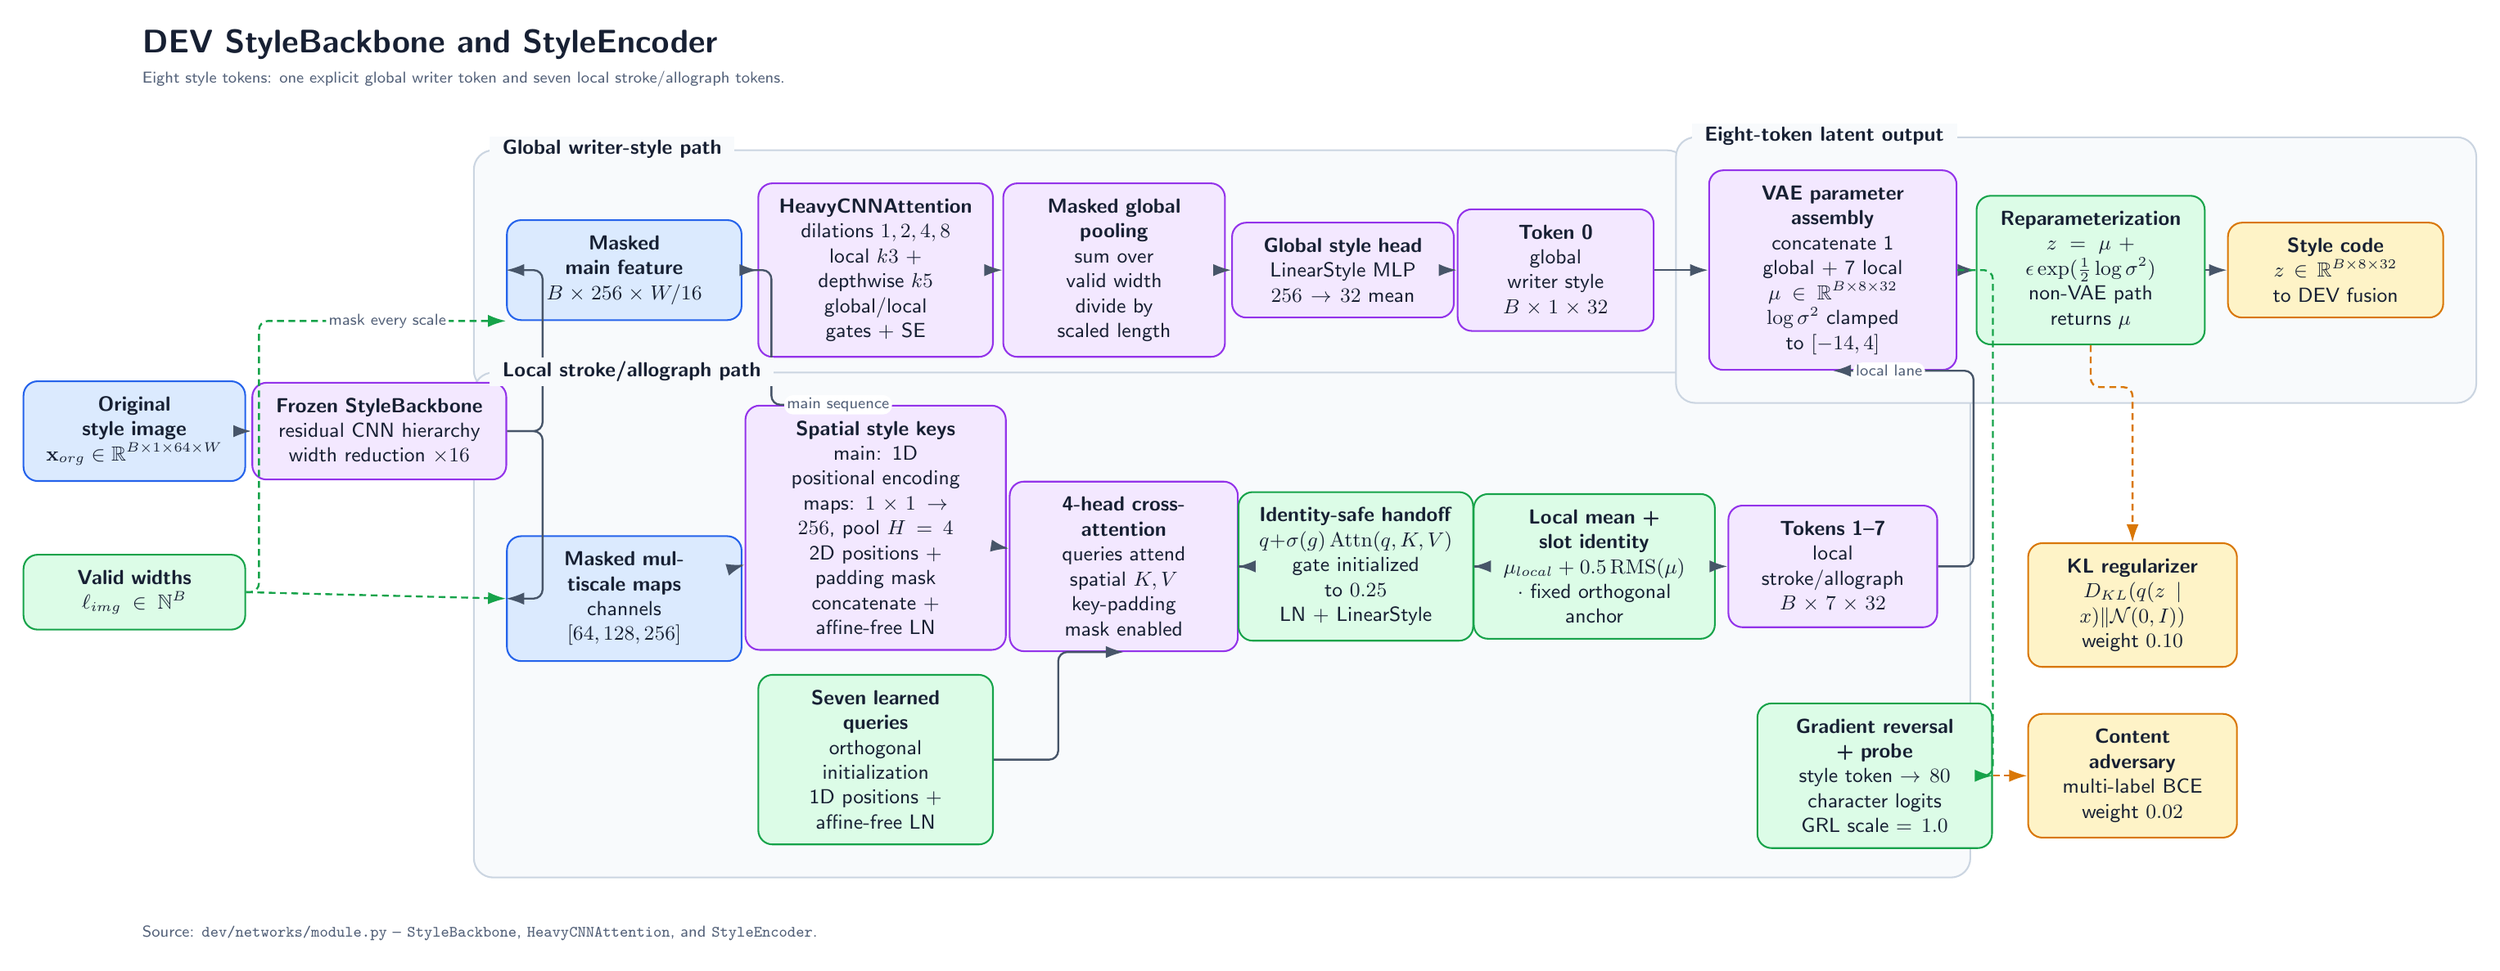
\begin{tikzpicture}[x=1cm,y=1cm]
  \node[font=\sffamily\bfseries\Large, text=DevInk, anchor=west]
    at (0,13.25) {DEV StyleBackbone and StyleEncoder};
  \node[devnote, anchor=west]
    at (0,12.72) {Eight style tokens: one explicit global writer token and seven local stroke/allograph tokens.};

  % Inputs and frozen backbone.
  \node[devinput, text width=2.8cm] (image) at (0,7.25)
    {\textbf{Original style image}\\$\mathbf{x}_{org}\in\mathbb{R}^{B\times1\times64\times W}$};
  \node[devstable, text width=2.8cm] (lengths) at (0,4.75)
    {\textbf{Valid widths}\\$\ell_{img}\in\mathbb{N}^{B}$};
  \node[devstyle, text width=3.3cm] (backbone) at (3.8,7.25)
    {\textbf{Frozen StyleBackbone}\\residual CNN hierarchy\\width reduction $\times16$};
  \node[devcontent, text width=3.0cm] (mainfeat) at (7.6,9.75)
    {\textbf{Masked main feature}\\$B\times256\times W/16$};
  \node[devcontent, text width=3.0cm] (multifeat) at (7.6,4.65)
    {\textbf{Masked multiscale maps}\\channels $[64,128,256]$};

  \draw[devflow] (image) -- (backbone);
  \draw[devflow] (backbone.east) -- ++(0.55,0) |- (mainfeat.west);
  \draw[devflow] (backbone.east) -- ++(0.55,0) |- (multifeat.west);
  \draw[devaux] (lengths.east) -- ++(0.20,0) |- node[devlabel,pos=0.76] {mask every scale} (mainfeat.south west);
  \draw[devaux] (lengths.east) -- (multifeat.west);

  % Global path.
  \node[devstyle, text width=3.0cm] (heavy) at (11.5,9.75)
    {\textbf{HeavyCNNAttention}\\dilations $1,2,4,8$\\local $k3$ + depthwise $k5$\\global/local gates + SE};
  \node[devstyle, text width=2.8cm] (globalpool) at (15.2,9.75)
    {\textbf{Masked global pooling}\\sum over valid width\\divide by scaled length};
  \node[devstyle, text width=2.8cm] (globalhead) at (18.75,9.75)
    {\textbf{Global style head}\\LinearStyle MLP\\$256\rightarrow32$ mean};
  \node[devstyle, text width=2.4cm] (globaltoken) at (22.05,9.75)
    {\textbf{Token 0}\\global writer style\\$B\times1\times32$};

  \draw[devflow] (mainfeat) -- (heavy);
  \draw[devflow] (heavy) -- (globalpool);
  \draw[devflow] (globalpool) -- (globalhead);
  \draw[devflow] (globalhead) -- (globaltoken);

  % Local key construction and local query path.
  \node[devstyle, text width=3.4cm] (keybuilder) at (11.5,5.75)
    {\textbf{Spatial style keys}\\main: 1D \mbox{positional} encoding\\maps: $1\times1\rightarrow256$, pool $H=4$\\2D positions + padding mask\\concatenate + affine-free LN};
  \node[devstable, text width=3.0cm] (queries) at (11.5,2.15)
    {\textbf{Seven learned queries}\\orthogonal initialization\\1D positions + affine-free LN};
  \node[devstyle, text width=2.9cm] (crossattn) at (15.35,5.15)
    {\textbf{4-head cross-attention}\\queries attend spatial $K,V$\\key-padding mask enabled};
  \node[devstable, text width=3.0cm] (queryres) at (18.95,5.15)
    {\textbf{Identity-safe handoff}\\$q+\sigma(g)\,\mathrm{Attn}(q,K,V)$\\gate \mbox{initialized} to $0.25$\\LN + LinearStyle};
  \node[devstable, text width=3.1cm] (anchors) at (22.65,5.15)
    {\textbf{Local mean + slot identity}\\$\mu_{local}+0.5\,\mathrm{RMS}(\mu)$\\$\cdot$ fixed \mbox{orthogonal} anchor};
  \node[devstyle, text width=2.6cm] (localtokens) at (26.35,5.15)
    {\textbf{Tokens 1--7}\\local stroke/allograph\\$B\times7\times32$};

  \draw[devflow] (mainfeat.east) -- ++(0.45,0) |- node[devlabel,pos=0.82] {main sequence} (keybuilder.north);
  \draw[devflow] (multifeat) -- (keybuilder);
  \draw[devflow] (queries.east) -- ++(1.0,0) |- (crossattn.south);
  \draw[devflow] (keybuilder) -- (crossattn);
  \draw[devflow] (crossattn) -- (queryres);
  \draw[devflow] (queryres) -- (anchors);
  \draw[devflow] (anchors) -- (localtokens);

  % Latent assembly is intentionally placed to the right, with separate lanes
  % for global and local tokens so their arrows never cross a block.
  \node[devstyle, text width=3.2cm] (latent) at (26.35,9.75)
    {\textbf{\mbox{VAE parameter} assembly}\\concatenate 1 global + 7 local\\$\mu\in\mathbb{R}^{B\times8\times32}$\\$\log\sigma^2$ clamped to $[-14,4]$};
  \node[devstable, text width=2.9cm] (sample) at (30.35,9.75)
    {\textbf{Reparameterization}\\$z=\mu+\epsilon\exp(\tfrac12\log\sigma^2)$\\non-VAE path returns $\mu$};
  \node[devloss, text width=2.7cm] (output) at (34.15,9.75)
    {\textbf{Style code}\\$z\in\mathbb{R}^{B\times8\times32}$\\to DEV fusion};

  \draw[devflow] (globaltoken) -- (latent);
  \draw[devflow] (localtokens.east) -- ++(0.55,0) |- node[devlabel,pos=0.80] {local lane} (latent.south);
  \draw[devflow] (latent) -- (sample);
  \draw[devflow] (sample) -- (output);

  % Training-only regularizers.
  \node[devstable, text width=3.0cm] (probe) at (27.0,1.9)
    {\textbf{\mbox{Gradient reversal} + probe}\\style token $\rightarrow80$ character logits\\GRL scale $=1.0$};
  \node[devloss, text width=2.6cm] (contentloss) at (31.0,1.9)
    {\textbf{Content adversary}\\multi-label BCE\\weight $0.02$};
  \node[devloss, text width=2.6cm] (klloss) at (31.0,4.55)
    {\textbf{KL regularizer}\\$D_{KL}(q(z\mid x)\Vert\mathcal{N}(0,I))$\\weight $0.10$};

  \draw[devlossflow] (sample.south) -- ++(0,-0.65) -| (klloss.north);
  \draw[devaux] (latent.east) -- ++(0.55,0) |- (probe.east);
  \draw[devlossflow] (probe) -- (contentloss);

  % Background groups are drawn after node placement but on the background layer.
  \begin{scope}[on background layer]
    \node[devgroup, fit=(mainfeat)(heavy)(globalpool)(globalhead)(globaltoken), inner sep=5mm] (globalgroup) {};
    \node[devgroup, fit=(multifeat)(keybuilder)(queries)(crossattn)(queryres)(anchors)(localtokens), inner sep=5mm] (localgroup) {};
    \node[devgroup, fit=(latent)(sample)(output), inner sep=5mm] (vaegroup) {};
  \end{scope}
  \node[devgrouptitle, anchor=west] at ($(globalgroup.north west)+(0.25,0)$)
    {Global writer-style path};
  \node[devgrouptitle, anchor=west] at ($(localgroup.north west)+(0.25,0)$)
    {Local stroke/allograph path};
  \node[devgrouptitle, anchor=west] at ($(vaegroup.north west)+(0.25,0)$)
    {Eight-token latent output};

  \node[devnote, anchor=west] at (0,-0.55)
    {Source: \texttt{dev/networks/module.py} -- \texttt{StyleBackbone}, \texttt{HeavyCNNAttention}, and \texttt{StyleEncoder}.};
\end{tikzpicture}
\end{document}

